% ============================================================
%  pgr-alnmap Technical Algorithm Report
%  Build:  pdflatex main.tex  (twice for references/TOC)
% ============================================================
\documentclass[11pt,a4paper]{article}

\usepackage[margin=2.5cm]{geometry}
\usepackage{amsmath,amssymb,amsthm}
\usepackage{algorithm}
\usepackage{algpseudocode}
\usepackage{booktabs}
\usepackage{array}
\usepackage{xcolor}
\usepackage{hyperref}
\usepackage{tikz}
\usepackage{pgfplots}
\pgfplotsset{compat=1.18}
\usetikzlibrary{arrows.meta, positioning, shapes.geometric, fit, backgrounds}
\usepackage{listings}
\usepackage{microtype}
\usepackage{parskip}
\usepackage{caption}
\usepackage{subcaption}
\usepackage{fancyhdr}
\usepackage{titlesec}
\usepackage{enumitem}

% ── Hyperref setup ──────────────────────────────────────────
\hypersetup{
  colorlinks = true,
  linkcolor  = blue!60!black,
  citecolor  = green!40!black,
  urlcolor   = blue!70!black,
  pdftitle   = {pgr-alnmap: Technical Algorithm Description},
  pdfauthor  = {PGR-TK Team},
}

% ── Listings (code) ─────────────────────────────────────────
\lstset{
  basicstyle   = \ttfamily\small,
  keywordstyle = \color{blue!70!black}\bfseries,
  commentstyle = \color{green!40!black}\itshape,
  stringstyle  = \color{red!60!black},
  frame        = single,
  breaklines   = true,
  numbers      = left,
  numberstyle  = \tiny\color{gray},
  xleftmargin  = 1.5em,
}

% ── Theorem environments ────────────────────────────────────
\newtheorem{definition}{Definition}[section]
\newtheorem{remark}{Remark}[section]

% ── Header / footer ─────────────────────────────────────────
\pagestyle{fancy}
\fancyhf{}
\rhead{\small pgr-alnmap Technical Report}
\lhead{\small PGR-TK}
\cfoot{\thepage}

% ── Title ───────────────────────────────────────────────────
\title{
  \textbf{pgr-alnmap: Technical Algorithm Description}\\[0.5em]
  \large Shimmer-Based Sparse Alignment, SV Candidate Detection,\\
         and Diploid Assembly Annotation
}
\author{PGR-TK Development Team}
\date{2026-04-07 \quad|\quad Branch: \texttt{aln\_map\_improvment}}

% ============================================================
\begin{document}
\maketitle
\tableofcontents
\newpage

% ============================================================
\section{Introduction}
\label{sec:intro}
% ============================================================

\texttt{pgr-alnmap} is the core alignment-and-annotation binary of the
PGR-TK (Pangenome Reference Toolkit) suite.
Given a reference genome and one or more assembly contigs, it produces:

\begin{itemize}[noitemsep]
  \item A chain-level sparse alignment of every contig against the reference.
  \item Fine-grained sequence alignments for each inter-shimmer gap, yielding
        SNP and short-indel calls.
  \item Structural variant (SV) candidate records wherever fine-grained alignment
        fails or the gap is too large.
  \item Duplication and overlap annotations on both the reference (target) and
        contig (query) coordinate axes.
  \item A self-contained SQLite database (\texttt{.alndb}) storing all of the above
        in a queryable schema.
\end{itemize}

The tool is designed for validating and annotating \emph{diploid, haplotype-resolved}
long-read assemblies (e.g., T2T-quality HiFi or ONT assemblies) against a curated
reference such as GRCh38.

\subsection{Inputs and Outputs}

\begin{table}[h]
\centering
\caption{Primary inputs and outputs of \texttt{pgr-alnmap}.}
\begin{tabular}{lll}
\toprule
\textbf{Direction} & \textbf{File / Format} & \textbf{Contents} \\
\midrule
Input  & \texttt{<ref>.fa[.gz]}    & Reference genome (FASTA, optionally PanSN format) \\
Input  & \texttt{<query>.fa[.gz]}  & Assembly contigs (FASTA) \\
Input  & \texttt{--preset} / flags & Algorithm parameters \\
\midrule
Output & \texttt{<prefix>.alndb}      & SQLite database (full results) \\
Output & \texttt{<prefix>.alnmap}     & Text alignment records \\
Output & \texttt{<prefix>.svcnd.bed}  & SV candidates, reference coordinates \\
Output & \texttt{<prefix>.ctgsv.bed}  & SV candidates, contig coordinates \\
Output & \texttt{<prefix>.svcnd.seqs} & Sequence pairs at SV sites \\
Output & \texttt{<prefix>.vcf}        & Small variant calls \\
Output & \texttt{<prefix>.ctgmap.bed} & Contig placement regions (BED) \\
Output & \texttt{<prefix>.ctgmap.json}& Contig placement records (JSON) \\
\bottomrule
\end{tabular}
\end{table}

% ============================================================
\section{Shimmer Index and Sparse Hit Finding}
\label{sec:shimmer}
% ============================================================

\subsection{Shimmers (Sparse K-mers)}

A \emph{shimmer} is a two-stage sparse $k$-mer anchor.
The construction proceeds as follows:

\begin{enumerate}
  \item \textbf{Stage 1 — window minimizers.}
        Standard $(w, k)$-minimizers are extracted from the sequence:
        for each window of $w$ consecutive $k$-mers, the lexicographically
        smallest canonical $k$-mer (forward or reverse complement, whichever
        is smaller) is retained.

  \item \textbf{Stage 2 — double reduction.}
        The function \texttt{reduce\_shmmr} is applied \emph{twice} in
        succession to the Stage-1 minimizer list.
        Each call selects the minimum-valued element within a sliding window
        of size $r$ over the \emph{already-sparse} minimizer list.
        Applying the reduction twice with window $r$ achieves a sparsity
        roughly equivalent to a single pass with window $r^2$, while the
        two-pass design ensures boundary stability.
\end{enumerate}

\begin{definition}[Shimmer]
  Given parameters $(w, k, r)$, a position $p$ in sequence $S$ is a shimmer if:
  \begin{enumerate}[noitemsep]
    \item The canonical $k$-mer at $p$ is the minimum in its $(w,k)$-minimizer
          window (Stage 1), and
    \item It survives both passes of \texttt{reduce\_shmmr} with window $r$
          (Stage 2) — i.e.\ it is the minimum within a window of $r$ Stage-1
          minimizers in both reduction sweeps.
  \end{enumerate}
\end{definition}

\begin{remark}
  The reduction factor $r$ controls sparsity at the second level: larger $r$
  yields fewer shimmers per kilobase and faster (but less sensitive) alignment.
  Valid values are $1 \leq r < 13$ (enforced by assertion in the source).
  With $r=1$ no reduction is applied and all Stage-1 minimizers are retained.
  Additionally, shimmers are filtered by a minimum inter-shimmer spacing
  (\texttt{min\_span}): a shimmer is discarded if the distance to either its
  predecessor or successor is below \texttt{min\_span}, preventing dense
  clusters in low-complexity regions.
\end{remark}

\subsection{Reference Index Construction}

The reference FASTA is loaded and indexed once per run:

\begin{algorithm}[H]
\caption{Reference shimmer index construction}
\begin{algorithmic}[1]
\Require Reference sequences $\mathcal{T}$, parameters $(w,k,r,\text{min\_span})$
\Ensure Hash map $\mathcal{I}$: shimmer hash $\to$ list of (seq\_id, pos, strand)
\ForAll{sequence $T \in \mathcal{T}$}
  \State Extract Stage-1 minimizers from $T$ with $(w,k)$
  \State Apply \texttt{reduce\_shmmr} twice with window $r$ $\to$ shimmer list $\mathcal{S}_T$
  \State Filter by \texttt{min\_span}: remove shimmers too close to neighbours
  \ForAll{consecutive shimmer pair $(s_i, s_{i+1})$ in $\mathcal{S}_T$}
    \State $h \gets H(s_i, s_{i+1})$  \Comment{Paired-shimmer hash}
    \State $\mathcal{I}[h].\text{append}((\text{seq\_id}, s_i.\text{pos}, \text{strand}))$
  \EndFor
\EndFor
\State Filter high-frequency entries: remove $h$ where $|\mathcal{I}[h]| > \text{max\_count}$
\end{algorithmic}
\end{algorithm}

\subsection{Query Hit Retrieval}

For each query contig, shimmers are extracted and looked up in $\mathcal{I}$:

\begin{algorithm}[H]
\caption{Query shimmer hit retrieval}
\begin{algorithmic}[1]
\Require Query contig $Q$, index $\mathcal{I}$, frequency thresholds
\Ensure Set of fragment hits $\mathcal{H}$
\State Extract shimmers from $Q$; build query shimmer list $\mathcal{S}_Q$
\ForAll{consecutive shimmer pair $(s_i, s_{i+1})$ in $\mathcal{S}_Q$}
  \State $h \gets H(s_i, s_{i+1})$
  \If{$h \in \mathcal{I}$ and $|\mathcal{I}[h]| \leq \text{max\_count}$}
    \ForAll{hit $(t\_\text{id}, t\_\text{pos}, t\_\text{strand}) \in \mathcal{I}[h]$}
      \State Emit \textbf{FragmentHit}: $(t\_\text{id},\; t\_\text{pos},\; t\_\text{pos}+\Delta_t,\;
                                          q\_\text{pos},\; q\_\text{pos}+\Delta_q,\; \text{strand})$
    \EndFor
  \EndIf
\EndFor
\end{algorithmic}
\end{algorithm}

% ============================================================
\section{Sparse Alignment Chain Building}
\label{sec:chain}
% ============================================================

\subsection{Hit Pair Representation}

Each fragment hit is converted to a \emph{HitPair}:
\[
  \bigl((q_s,\, q_e,\, \text{orient}_q),\; (t_s,\, t_e,\, \text{orient}_t)\bigr)
\]
capturing aligned intervals on both the query and target with their strands.

\subsection{Dynamic Programming Chaining}

Chains are built by a banded DP over the sorted hit sequence.
Let $\mathcal{P} = \{p_1, p_2, \ldots, p_n\}$ be the hits sorted by
$(t\_\text{seq\_id},\; t_s)$.

\begin{definition}[Chain score]
  For a chain ending at hit $p_i$, the DP score is:
  \[
    \mathrm{DP}[i] = \max_{j < i,\; \text{compat}(j,i)}
      \Bigl(\mathrm{DP}[j] + \mathrm{score}(p_i) - \mathrm{gap\_pen}(p_j, p_i)\Bigr)
  \]
  where $\mathrm{score}(p_i) = p_i.t_e - p_i.t_s$ (span on target) and
  \[
    \mathrm{gap\_pen}(p_j, p_i) = \lambda \cdot
      \max\bigl(|{(t_s^i - t_e^j)} - (q_s^i - q_e^j)|\,,\; 0\bigr)
  \]
  with gap penalty factor $\lambda$ (default 0.025).
\end{definition}

Compatibility $\mathrm{compat}(j, i)$ requires:
\begin{itemize}[noitemsep]
  \item Same target sequence and same query sequence.
  \item Consistent strand orientation.
  \item $t_s^i > t_e^j$ (non-overlapping on target, in order).
  \item $q_s^i > q_e^j$ (non-overlapping on query, in order).
  \item Gap $t_s^i - t_e^j \leq \text{max\_gap}$ (default 100\,kbp).
\end{itemize}

The DP window is limited to \texttt{max\_aln\_chain\_span} predecessors
(default 8) for efficiency.

\begin{algorithm}[H]
\caption{\textsc{SparseAln}: chain building by DP}
\begin{algorithmic}[1]
\Require Hit list $\mathcal{P}$ sorted by $(t\_\text{id}, t_s)$, parameters $\lambda$, max\_gap
\Ensure List of alignment chains $\mathcal{C}$
\State Initialise $\mathrm{DP}[i] \gets \mathrm{score}(p_i)$, $\mathrm{pred}[i] \gets \text{nil}$
\For{$i \gets 1$ to $n$}
  \For{$j \gets \max(0,\, i - \text{max\_aln\_chain\_span})$ to $i-1$}
    \If{$\mathrm{compat}(j, i)$}
      \State $s \gets \mathrm{DP}[j] + \mathrm{score}(p_i) - \mathrm{gap\_pen}(p_j, p_i)$
      \If{$s > \mathrm{DP}[i]$}
        \State $\mathrm{DP}[i] \gets s$;\quad $\mathrm{pred}[i] \gets j$
      \EndIf
    \EndIf
  \EndFor
\EndFor
\State Backtrack from highest-scoring, non-suppressed $i$ to reconstruct chains
\State \Return $\mathcal{C}$
\end{algorithmic}
\end{algorithm}

Non-overlapping chains are extracted greedily in decreasing score order;
chains whose intervals are subsumed by a higher-scoring chain are suppressed.

% ============================================================
\section{Fine-Grained Sequence Alignment and Variant Calling}
\label{sec:finealn}
% ============================================================

\subsection{Inter-Shimmer Gap Resolution}

For each consecutive hit pair $(p_j, p_k)$ within a chain, the \emph{gap region}
(target interval $[t_e^j, t_s^k]$ and query interval $[q_e^j, q_s^k]$)
is extracted with $k$-bp flanking padding and aligned at the nucleotide level.

Quality pre-checks reject a gap before alignment:
\begin{enumerate}[noitemsep]
  \item \textbf{FailShortSeq}: either interval $< 16$\,bp.
  \item \textbf{FailEndMatch}: the $k$-bp flanking regions do not match exactly.
  \item \textbf{FailLengthDiff}: $|L_t - L_q| \geq 128$\,bp
        (for the Smith-Waterman path; WFA handles larger diffs).
\end{enumerate}

Gaps passing pre-checks are aligned using:
\begin{itemize}[noitemsep]
  \item \textbf{WFA} (Wavefront Alignment Algorithm) for the general case.
  \item \textbf{Smith-Waterman} for regions where $|L_t - L_q| < \text{max\_sw\_aln\_size}$.
\end{itemize}

Alignment scoring: mismatch penalty $= 1$, gap-open $= 4$, gap-extend $= 4$.

\subsection{Variant Extraction}

From the CIGAR-like alignment output, variant segments are extracted:

\begin{algorithm}[H]
\caption{Variant extraction from alignment}
\begin{algorithmic}[1]
\Require Alignment CIGAR between target $T[t_s\ldots t_e]$ and query $Q[q_s\ldots q_e]$
\Ensure Variant list $\mathcal{V}$
\State Walk CIGAR operations, tracking $t\_\text{pos}$, $q\_\text{pos}$
\ForAll{non-match run of length $\ell$}
  \If{$\ell = 1$ and both ref and alt are single bases}
    \State Emit \textbf{SNP}: $(t\_\text{pos},\; \text{ref\_base},\; \text{alt\_base})$
  \ElsIf{insertion ($q$-only)}
    \State Emit \textbf{Insertion}: $(t\_\text{pos},\; \varepsilon,\; Q[q\_\text{pos}\ldots q\_\text{pos}+\ell])$
  \ElsIf{deletion ($t$-only)}
    \State Emit \textbf{Deletion}: $(t\_\text{pos},\; T[t\_\text{pos}\ldots t\_\text{pos}+\ell],\; \varepsilon)$
  \EndIf
\EndFor
\end{algorithmic}
\end{algorithm}

\subsection{Match Block Recording}

Gaps that align with zero variants are recorded as \textbf{M-blocks}
(perfect match regions).  These are the foundation for the transcript
liftover step in \texttt{pgr-liftover-gtf}.

% ============================================================
\section{SV Candidate Classification}
\label{sec:svcnd}
% ============================================================

\subsection{Primary SV Candidates}

A gap region that fails any pre-check or whose alignment fails becomes an
\textbf{SV candidate} block.  The failure type is recorded as a diff-type code:

\begin{table}[h]
\centering
\caption{SV candidate diff-type codes.}
\begin{tabular}{cll}
\toprule
\textbf{Code} & \textbf{Name} & \textbf{Condition} \\
\midrule
\texttt{A} & FailAln        & WFA or SW alignment did not converge \\
\texttt{E} & FailEndMatch   & Flanking $k$-bp regions do not match \\
\texttt{S} & FailShortSeq   & Gap interval $< 16$\,bp \\
\texttt{L} & FailLengthDiff & $|L_t - L_q| \geq 128$\,bp (SW path) \\
\bottomrule
\end{tabular}
\end{table}

\subsection{Target-Axis Structural Annotations}
\label{sec:target-annot}

After all chains are computed, the reference (target) coordinate axis is
analysed per chromosome.
Contig alignments are sorted by $t_s$ and scanned left-to-right:

\begin{itemize}
  \item \textbf{TG (Target Gap)}: A non-mapped reference interval between two
        consecutive contig alignments $[t_e^{(i)}, t_s^{(i+1)}]$.
        The gap suggests a sequence present in the reference but absent or
        rearranged in the assembly.
  \item \textbf{TD (Target Duplicate)}: A new contig alignment whose target
        interval $[t_s^{(j)}, t_e^{(j)}]$ is \emph{fully contained within}
        the interval of a previous alignment.
        Indicates that two different assembly contigs map to the same reference
        region (segmental duplication or assembly redundancy).
  \item \textbf{TO (Target Overlap)}: A new alignment that \emph{partially}
        overlaps the target interval of a previous alignment.
\end{itemize}

\begin{figure}[h]
\centering
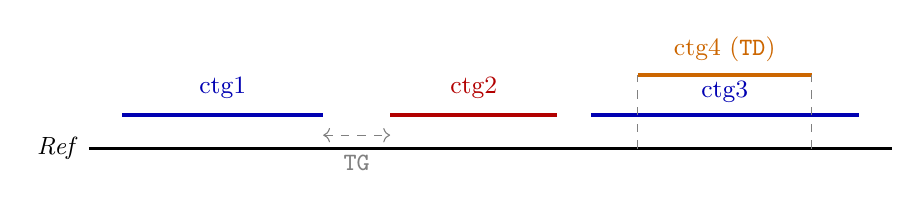
\begin{tikzpicture}[scale=0.85, font=\small]
  % Reference bar
  \draw[thick] (0,0) -- (12,0);
  \node[left] at (0,0) {\textit{Ref}};

  % TG gap
  \draw[blue!70!black, very thick] (0.5,0.5) -- (3.5,0.5);
  \draw[red!70!black,  very thick] (4.5,0.5) -- (7,0.5);
  \draw[<->, dashed, gray] (3.5,0.2) -- (4.5,0.2);
  \node[below, gray] at (4,0.05) {\texttt{TG}};
  \node[above, blue!70!black] at (2,0.6) {ctg1};
  \node[above, red!70!black]  at (5.75,0.6) {ctg2};

  % TD (contained)
  \draw[blue!70!black, very thick] (7.5,0.5) -- (11.5,0.5);
  \draw[orange!80!black, very thick] (8.2,1.1) -- (10.8,1.1);
  \node[above, blue!70!black] at (9.5,0.55) {ctg3};
  \node[above, orange!80!black] at (9.5,1.15) {ctg4 (\texttt{TD})};
  \draw[dashed, gray] (8.2,0) -- (8.2,1.1);
  \draw[dashed, gray] (10.8,0) -- (10.8,1.1);
\end{tikzpicture}
\caption{Illustration of \texttt{TG} (target gap between ctg1 and ctg2)
         and \texttt{TD} (ctg4 fully contained within ctg3's reference span).}
\end{figure}

\subsection{Query-Axis Structural Annotations}

The symmetric analysis on the contig (query) coordinate axis produces:

\begin{itemize}
  \item \textbf{QG (Query Gap)}: An unaligned region within a contig between
        two consecutive reference alignments.
        Indicates a sequence in the assembly that has no reference counterpart
        at that position.
  \item \textbf{QD (Query Duplicate)}: A reference alignment fully contained
        within a previous one on the same contig.
  \item \textbf{QO (Query Overlap)}: A reference alignment partially overlapping
        a previous one on the same contig.
\end{itemize}

\subsection{SV Candidate Overlay}

Primary SV candidate blocks are overlaid against the target-duplicate (\texttt{TD})
and target-overlap (\texttt{TO}) interval sets to yield three subtypes in the output:

\begin{table}[h]
\centering
\caption{SV candidate subtypes in the \texttt{.svcnd.bed} output.}
\begin{tabular}{lll}
\toprule
\textbf{Subtype} & \textbf{Short} & \textbf{Meaning} \\
\midrule
SV candidate (plain)     & \texttt{SV}  & Lies in a non-redundant reference region \\
SV candidate (duplicate) & \texttt{SV\_D} & Overlaps a TD (target duplicate) interval \\
SV candidate (overlap)   & \texttt{SV\_O} & Overlaps a TO (target overlap) interval \\
\bottomrule
\end{tabular}
\end{table}

% ============================================================
\section{Output Database Schema (\texttt{.alndb})}
\label{sec:schema}
% ============================================================

All results are stored in a single SQLite database.
The schema is designed so that the most common queries
(e.g., ``all M-blocks on chr1 overlapping a gene'') can be satisfied
with a single indexed join.

\begin{table}[h]
\centering
\caption{Tables in the \texttt{.alndb} SQLite database.}
\begin{tabular}{lp{9cm}}
\toprule
\textbf{Table} & \textbf{Contents} \\
\midrule
\texttt{run\_params}   & Key-value store of all algorithm parameters used \\
\texttt{sequences}     & Names and lengths of all target and query sequences \\
\texttt{chains}        & One row per alignment chain (top-level contig placement) \\
\texttt{blocks}        & M-blocks and SV candidate blocks within each chain \\
\texttt{variants}      & SNP and short-indel calls with ref/alt sequences \\
\texttt{ctgmap}        & Contig-level placement summary (one row per contig) \\
\texttt{sv\_candidates}& High-level SV candidate regions on the reference axis \\
\texttt{ctgsv}         & SV candidate regions on the query (contig) axis \\
\texttt{sv\_sequences} & Reference and query sequences flanking each SV site \\
\bottomrule
\end{tabular}
\end{table}

The database is written with WAL journalling mode and normal synchronous mode
for a balance of write throughput and crash safety.
All inserts use parameterised prepared statements.

% ============================================================
\section{Algorithm Parameters and Presets}
\label{sec:params}
% ============================================================

\begin{table}[h]
\centering
\caption{Preset parameter values.}
\begin{tabular}{lrrrrr}
\toprule
\textbf{Preset} & $w$ & $k$ & $r$ & \text{min\_span} & \text{max\_sw\_aln\_size} \\
\midrule
\texttt{fast}    & 80 & 55 & 4 & 64 & 1\,024 \\
\texttt{default} & 48 & 55 & 2 & 16 & 1\,024 \\
\texttt{detail}  & 48 & 55 & 2 & 16 & 32\,864 \\
\bottomrule
\end{tabular}
\end{table}

\begin{table}[h]
\centering
\caption{Global parameters (not preset-specific).}
\begin{tabular}{lll}
\toprule
\textbf{Parameter} & \textbf{Default} & \textbf{Description} \\
\midrule
\texttt{max\_gap}              & 100\,000 bp & Maximum gap in DP chaining \\
\texttt{max\_aln\_chain\_span} & 8           & DP predecessor window size \\
\texttt{gap\_penalty\_factor}  & 0.025       & Gap penalty factor $\lambda$ \\
\texttt{mismatch\_penalty}     & 1           & Nucleotide mismatch cost \\
\texttt{gap\_open}             & 4           & Affine gap open penalty \\
\texttt{gap\_extend}           & 4           & Affine gap extension penalty \\
\bottomrule
\end{tabular}
\end{table}

\begin{remark}
  The \texttt{detail} preset increases \texttt{max\_sw\_aln\_size} to 32\,864\,bp,
  allowing Smith-Waterman alignment over much longer gap intervals at the cost
  of substantially longer runtime.  It is recommended only for targeted
  re-analysis of specific loci.
\end{remark}

% ============================================================
\section{Pipeline Overview}
\label{sec:overview}
% ============================================================

Figure~\ref{fig:pipeline} shows the end-to-end data flow.

\begin{figure}[h]
\centering
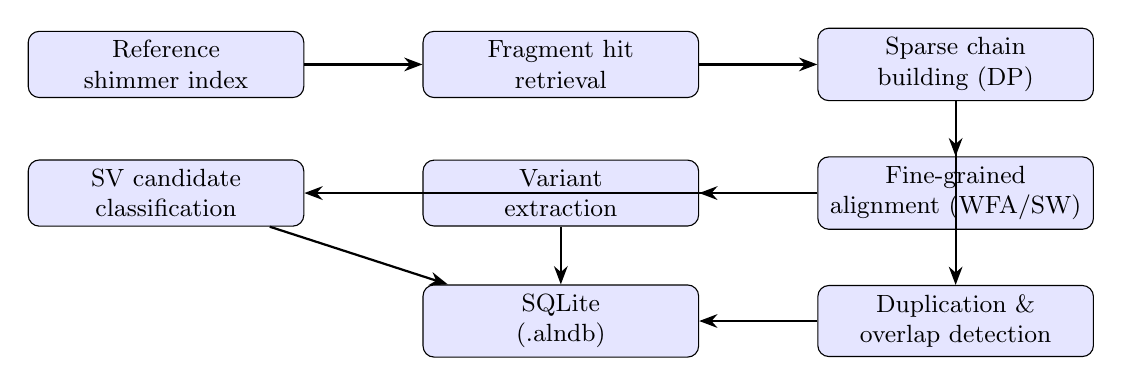
\begin{tikzpicture}[
  node distance = 0.7cm and 1.5cm,
  box/.style  = {rectangle, rounded corners, draw, fill=blue!10,
                 minimum width=3.5cm, minimum height=0.8cm,
                 align=center, font=\small},
  out/.style  = {rectangle, rounded corners, draw, fill=orange!15,
                 minimum width=3.5cm, minimum height=0.7cm,
                 align=center, font=\footnotesize},
  arr/.style  = {-Stealth, thick},
]

\node[box] (idx)  {Reference\\shimmer index};
\node[box, right=of idx] (hit) {Fragment hit\\retrieval};
\node[box, right=of hit] (chain) {Sparse chain\\building (DP)};
\node[box, below=of chain] (fine) {Fine-grained\\alignment (WFA/SW)};
\node[box, left=of fine] (var) {Variant\\extraction};
\node[box, left=of var] (svcnd) {SV candidate\\classification};
\node[box, below=of fine] (dup) {Duplication \&\\overlap detection};
\node[box, left=of dup] (db) {SQLite\\(.alndb)};

\draw[arr] (idx)   -- (hit);
\draw[arr] (hit)   -- (chain);
\draw[arr] (chain) -- (fine);
\draw[arr] (fine)  -- (var);
\draw[arr] (fine)  -- (svcnd);
\draw[arr] (chain) -- (dup);
\draw[arr] (var)   -- (db);
\draw[arr] (svcnd) -- (db);
\draw[arr] (dup)   -- (db);

\end{tikzpicture}
\caption{Data flow in \texttt{pgr-alnmap}.}
\label{fig:pipeline}
\end{figure}

% ============================================================
\section{Complexity Notes}
\label{sec:complexity}
% ============================================================

\begin{itemize}
  \item \textbf{Index construction}: $O(L_T / r)$ shimmer pairs for a reference of
        length $L_T$, stored in a hash map.  Memory proportional to index size.

  \item \textbf{Hit retrieval per contig}: $O(L_Q / r \cdot \bar{h})$ where $\bar{h}$
        is the mean number of reference hits per shimmer.  Rare shimmers
        (\texttt{max\_count} filter) bound $\bar{h}$ in practice.

  \item \textbf{Chaining DP}: $O(n \cdot \text{max\_aln\_chain\_span})$ per contig,
        where $n$ is the number of hits.  With the default window of 8 this is
        effectively linear.

  \item \textbf{Fine-grained alignment}: WFA runs in $O((s+1)(L+1))$ time where
        $s$ is the edit distance and $L$ is the gap length.
        The \texttt{FailLengthDiff} guard prevents runaway alignment on
        large indels.

  \item \textbf{Duplication/overlap detection}: $O(n_b \log n_b)$ per chromosome
        where $n_b$ is the number of alignment blocks, dominated by sorting.
\end{itemize}

% ============================================================
\section{Downstream Usage}
\label{sec:downstream}
% ============================================================

The \texttt{.alndb} produced by \texttt{pgr-alnmap} is consumed by several
downstream PGR-TK tools:

\begin{itemize}
  \item \textbf{pgr-liftover-gtf}: Loads M-blocks from \texttt{blocks} to map
        exon coordinates from the reference onto assembly contigs, producing
        the \texttt{\_liftover.db} transcript annotation database.
  \item \textbf{pgr-generate-diploid-vcf}: Merges variants from two haplotype
        \texttt{.alndb} files into a phased diploid VCF.
  \item \textbf{pgr-generate-chr-aln-plot}: Reads chains and blocks to render
        whole-genome dot-plot alignment HTML reports.
  \item \textbf{generate\_e2e\_report.py}: Reads \texttt{sv\_candidates} and
        \texttt{ctgsv} for the SV summary report and gene-impact annotation.
\end{itemize}

% ============================================================
\section*{Acknowledgements}
\addcontentsline{toc}{section}{Acknowledgements}
% ============================================================

This document was prepared by the PGR-TK development team.
Algorithm design and implementation by Jason Chin.
Technical report assistance by Claude Code (Anthropic).

% ============================================================
\end{document}
